%% ----------------------------------------------------
%%              NOTES-TEMPLATE
%% ----------------------------------------------------
\documentclass[12pt,a4paper]{article}
%\usepackage[margin=1in]{geometry}
\usepackage[landscape]{geometry}
\usepackage{graphicx}
\geometry{legalpaper, landscape}
\graphicspath{ {./images/} }
\usepackage{amsmath}
\pagenumbering{gobble}
\usepackage{amssymb}
\usepackage{gensymb}
\usepackage{mathrsfs}
\usepackage{multicol}
\usepackage{tikz}
\usetikzlibrary{shapes.geometric,positioning,arrows}
\usepackage[autostyle]{csquotes}
\renewcommand{\baselinestretch}{0.8}
\setlength{\columnsep}{1cm}
\usepackage{xcolor} % font coloring
\usepackage{sectsty}
%\sectionfont{\color{red}}  % sets colour of sections
\setlength{\parindent}{-1em}
%\sectionfont{\color{red}}  % sets colour of sections
%\subsectionfont{\color{purple}}
%\subsubsectionfont{\color{blue}}

%% math macros
\newcommand{\R}{\mathbb{R}}
\newcommand{\Z}{\mathbb{Z}}
\newcommand{\N}{\mathbb{N}}
\newcommand{\C}{\mathbb{C}}
\newcommand{\Q}{\mathbb{Q}}
\newcommand{\W}{\mathbb{W}}
\newtheorem{thm}{Theorem}
\newtheorem{defn}{Definition}
\newtheorem{conv}{Convention}
\newtheorem{rem}{Remark}
\newtheorem{lem}{Lemma}
\newtheorem{cor}{Corollary}
\newtheorem{ex}{Example}

%%% Coloring macros
\newcommand{\cred}[1]{\textcolor{red}{#1}}
\newcommand{\cblue}[1]{\textcolor{blue}{#1}}
\newcommand{\ccyan}[1]{\textcolor{cyan}{#1}}
\newcommand{\cgreen}[1]{\textcolor{green}{#1}}
\newcommand{\cyellow}[1]{\textcolor{yellow}{#1}}
\newcommand{\cpurple}[1]{\textcolor{purple}{#1}}
\newcommand{\corange}[1]{\textcolor{orange}{#1}}
%% custom colors
\definecolor{astral}{RGB}{46,116,181}
\definecolor{darkblue}{RGB}{50,76,168}
\definecolor{darkbrown}{RGB}{99,12,8}

\title{Proposed Hybrid Cryptosystem \vspace{-2em}}
%\author{Hamjak Debbarma}
\date{\today}
\linespread{0.5}

\tikzstyle{block} = [rectangle, draw, fill=blue!15, text width=5em, text centered, rounded corners, minimum height=4em]
\tikzstyle{Key} = [ellipse, draw, fill=red!30, node distance=3cm, minimum height=2em]
\tikzstyle{line} = [draw, very thick, color=black!50, -latex']
\tikzstyle{decision} = [diamond, draw, fill=blue!15, text centered, minimum height=2em]
\tikzstyle{egg} = [ellipse, draw, fill=green!30, node distance=4cm, minimum height=2em]
\begin{document}
  \maketitle

\subsection*{Encryption Process}
\begin{center}
	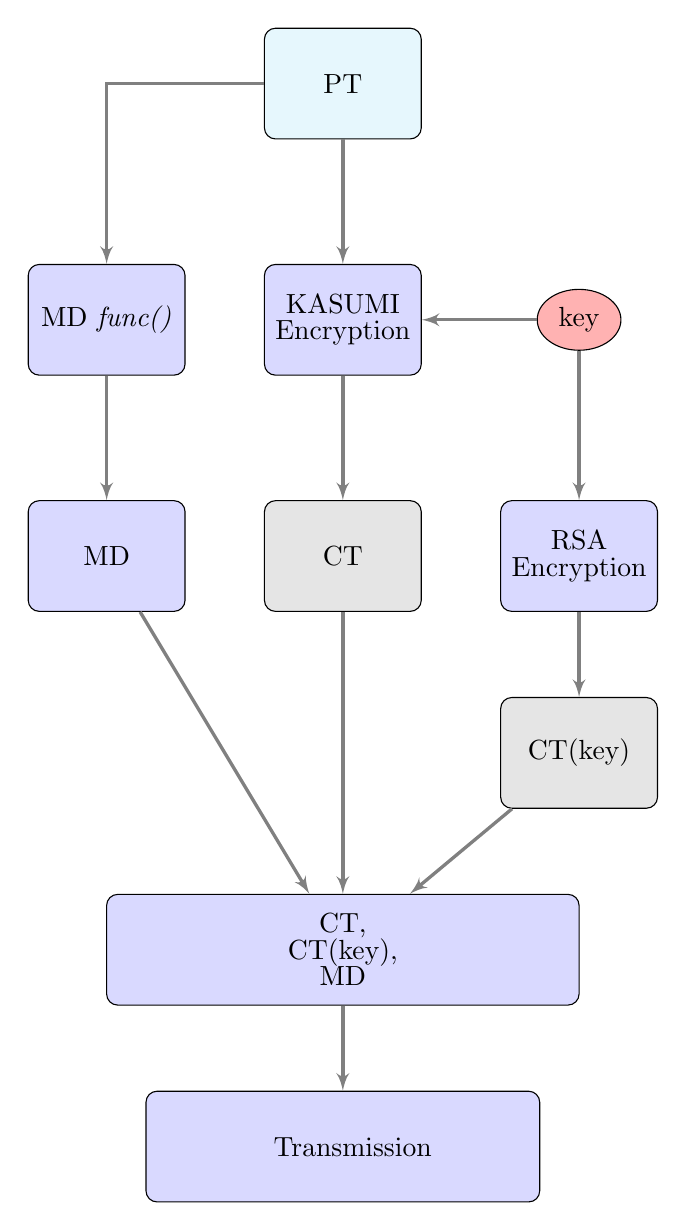
\begin{tikzpicture}
	%% PT Block
	\node [block, fill=cyan!10](PT){PT};
	%% KASUMI
	\node[block, below of=PT, node distance=3cm] (KC) {KASUMI Encryption};
	%% key block
	\node[Key, right of=KC, node distance=3cm](K) {key};
	%% CT Block
	\node[block, below of=KC,fill=gray!20, node distance=3cm](CT) {CT};
	%% MD function
	\node[block, left of=KC, node distance=3cm](MDF) {MD \textit{func()}};
	%% MD
	\node[block, below of=MDF, node distance=3cm](MD) {MD};
	%% RSA
	\node[block, right of=CT, node distance=3cm] (RSA) {RSA Encryption};
	%% send
	\node[block, below of=CT, node distance=5cm, minimum width=6cm] (Send) {CT, CT(key), MD};
	%% RSA CT
	\node[block, below of=RSA, fill=gray!20, node distance=2.5cm] (CT-key) {CT(key)};
	%% Transmission
	\node[block, below of=Send, node distance=2.5cm, minimum width=5cm] (Trans) {Transmission};
	%% edges
	\path[line](PT) -- (KC);
	\path[line](KC) -- (CT);
	\path[line](CT) -- (Send);
	\path[line](PT)-| (MDF);
	\path[line](MDF) -- (MD);
	\path[line](MD) -- (Send);
	\path[line](K) -- (RSA);
	\path[line](K) -- (KC);
	\path[line](RSA) -- (CT-key);
	\path[line](CT-key) -- (Send);
	\path[line](Send) -- (Trans);
	
	\end{tikzpicture}
\end{center}
  
  \subsection*{Decryption Process}
  \begin{center}
  	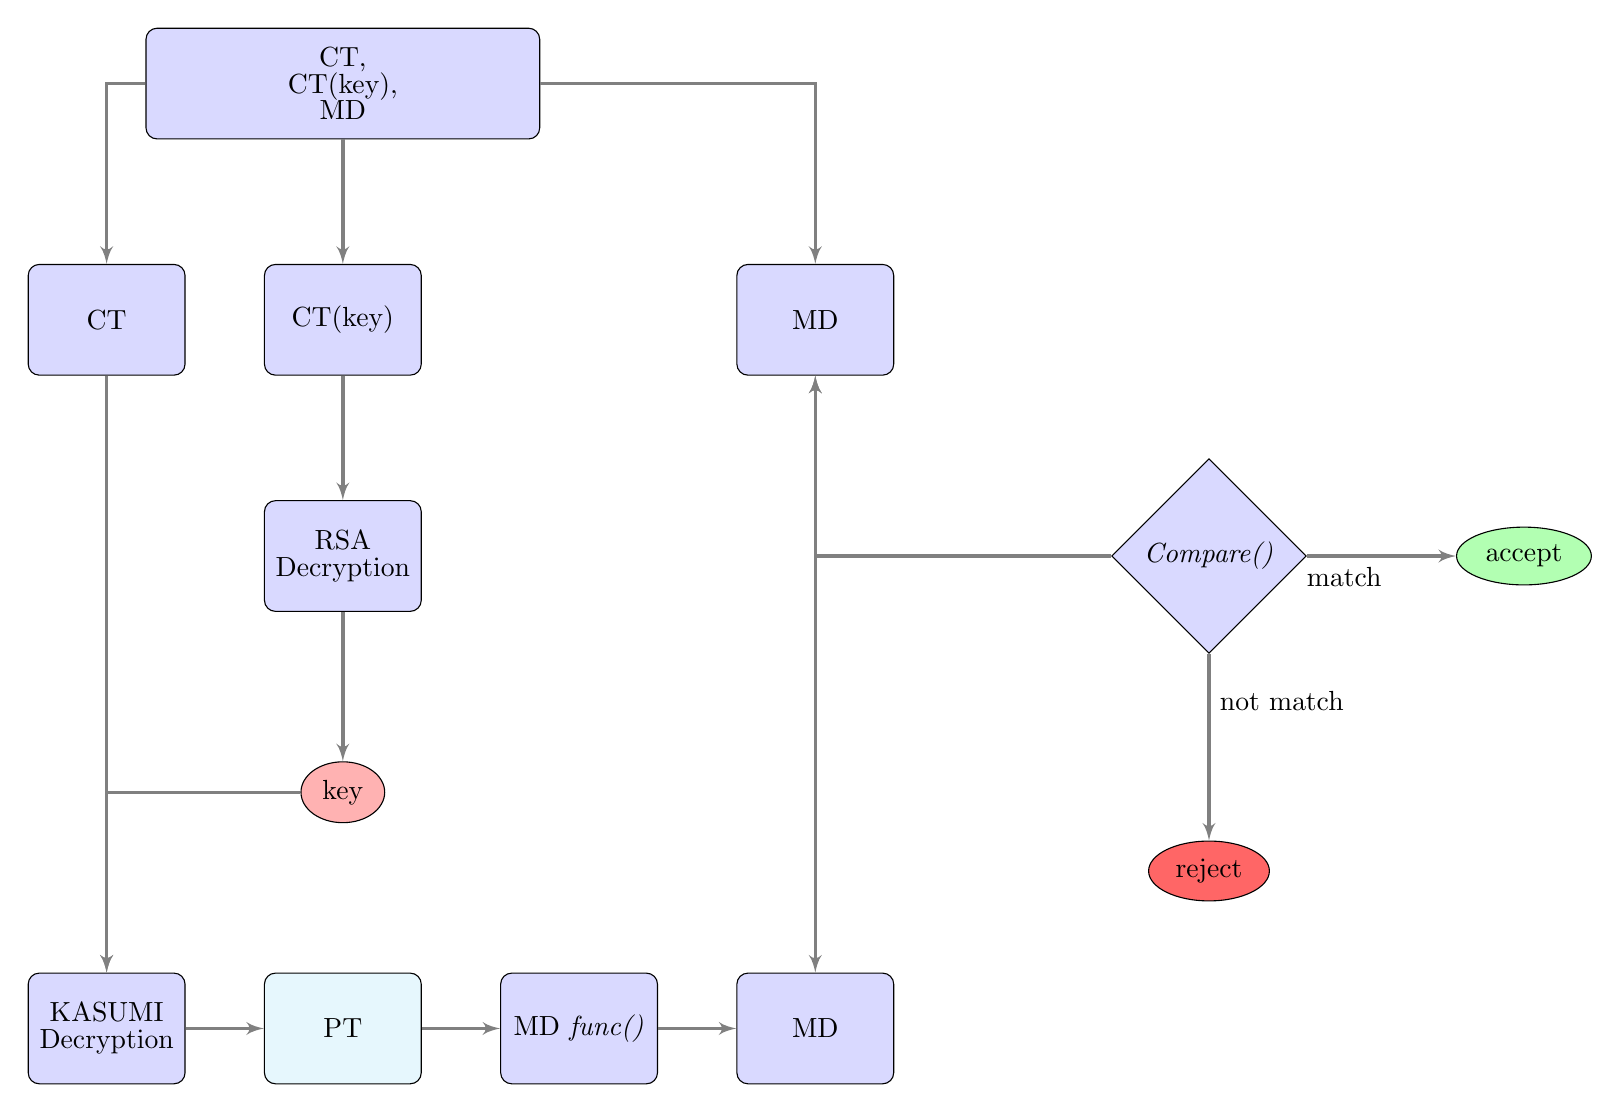
\begin{tikzpicture}
  	%% PT Block
  	\node [block, minimum width=5cm](R){CT, CT(key), MD};
  	%% KASUMI
  	\node[block, below of=R, node distance=3cm] (CT-k) {CT(key)};
  	%% key block
  	\node[block, right of=CT-k, node distance=6cm](MD) {MD};
  	%% CT Block
  	\node[block, left of=CT-k, node distance=3cm](CT-m) {CT};
  	%% MD function
  	\node[block, below of=CT-k, node distance=3cm](RSA-d) {RSA Decryption};
  	%% MD
  	\node[Key, below of=RSA-d, node distance=3cm](K) {key};
  	%% RSA
  	\node[block, below of=CT-m, node distance=9cm] (KCd) {KASUMI Decryption};
  	%% send
  	\node[block, right of=KCd, node distance=3cm, fill=cyan!10] (PT) {PT};
  	%% RSA CT
  	\node[block, right of=PT, node distance=3cm] (MDF) {MD \textit{func()}};
  	%% Transmission
  	\node[block, right of=MDF, node distance=3cm] (nMD) {MD};
  	\node[decision, right of=RSA-d, node distance=11cm] (cmp) {\textit{Compare()}};
  	\node[egg, right of=cmp] (y) {accept};
  	\node[egg, below of=cmp, fill=red!60] (n) {reject};
  	%% edges
  	\path[line](R) -| (CT-m);
  	\path[line](R) -| (MD);
  	\path[line](R) -- (CT-k);
  	\path[line](CT-k) -- (RSA-d);
  	\path[line, latex'-latex'](MD) -- (nMD);
  	\path[line](cmp) -| (MD);
  	\path[line](RSA-d) -- (K);
	\path[line](CT-m) -- (KCd);
	\path[line](K) -| (KCd);
	\path[line](KCd) -- (PT);
 	\path[line](PT) -- (MDF);
 	\path[line](MDF) -- (nMD);
 	%%\path[line](cmp) -- (y);
 	\path[line](cmp) -- node[below, near start, color=black]{match}(y);
 	\path[line](cmp) -- node[right, near start, color=black]{not match}(n);
  	\end{tikzpicture}
  \end{center}
  
  
\end{document}
